\section*{Binary search trees%
\TAGS{bst}}

A binary tree, like a linked list, is a recursive data structure. The
only difference is that a node can have 0, 1, or 2 children, which can
be other nodes or leaves. A leaf is a type of node that has no
children.

\begin{lstlisting}
typedef struct tree_node tree;
struct tree_node {
  elem data;
  tree* left;
  tree* right;
};
\end{lstlisting}
We call \lstinline'left' and \lstinline'right' subtrees.

A \emph{binary search tree (BST)} has an additional invariant, the
\emph{ordering invariant}. For a node with key $k$, all elements
in the left subtree must have keys that are strictly less than than
$k$, and all elements in the right subtree must have keys that are
strictly greater than $k$ (By this definition, we do not allow
duplicate keys).

\checkpoint*{\TAGS{bst, ds-invariant}}
Circle all of the nodes that contain keys that violate the ordering invariant.

\begin{center}
\begin{tikzpicture}
  \node (0) {5};

  \node[node distance=1.5cm] (1) [below left of=0] {-2};

  \node (2) [below left of=1] {-8};
  \node (3) [below right of=1] {5};

  \node (4) [below right of=2] {-3};

  \node[node distance=1.5cm] (5) [below right of=0] {8};

  \node (6) [below left of=5] {2};
  \node (7) [below right of=5] {17};

  \node (8) [below left of=7] {11};
  \node (9) [below right of=7] {9};

  \path[]
  (0) edge (1)
      edge (5)

  (1) edge (2)
      edge (3)

  (5) edge (6)
      edge (7)

  (2) edge (4)

  (7) edge (8)
      edge (9);
\end{tikzpicture}
\end{center}

\begin{solution}
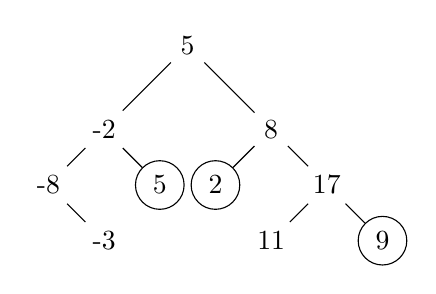
\begin{tikzpicture}
  \node (0) {5};

  \node[node distance=1.5cm] (1) [below left of=0] {-2};

  \node (2) [below left of=1] {-8};
  \node[circle, draw] (3) [below right of=1] {5};

  \node (4) [below right of=2] {-3};

  \node[node distance=1.5cm] (5) [below right of=0] {8};

  \node[circle, draw] (6) [below left of=5] {2};
  \node (7) [below right of=5] {17};

  \node (8) [below left of=7] {11};
  \node[circle, draw] (9) [below right of=7] {9};

  \path[]
  (0) edge (1)
      edge (5)

  (1) edge (2)
      edge (3)

  (5) edge (6)
      edge (7)

  (2) edge (4)

  (7) edge (8)
      edge (9);
\end{tikzpicture}
\end{solution}
